% Figure: RQ1 F1 Comparison (Gemini Flash Lite, n=200)
\begin{figure*}[t]
\centering
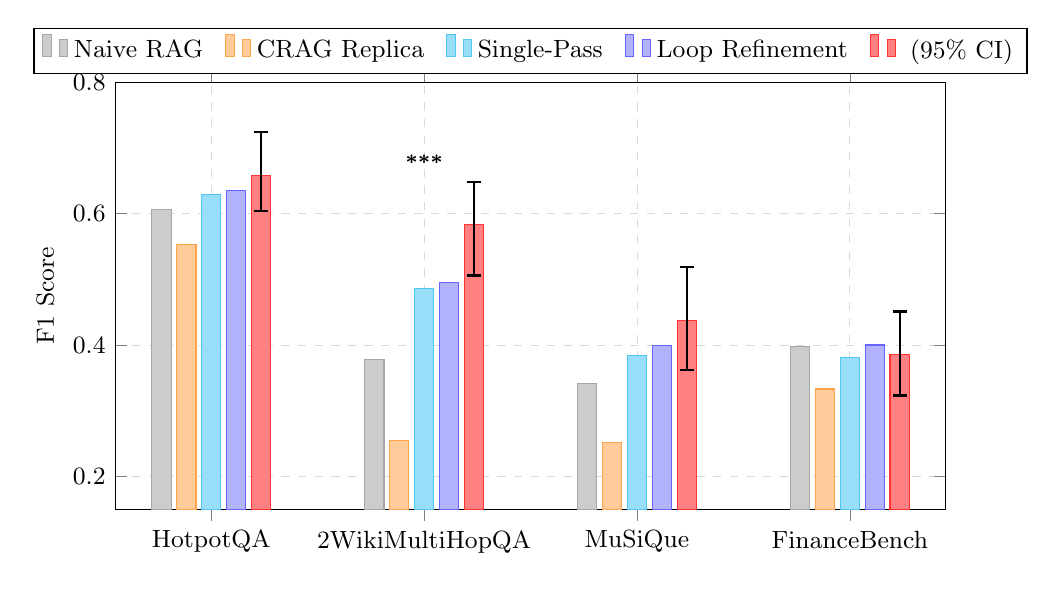
\begin{tikzpicture}
\begin{axis}[
    ybar,
    bar width=7pt,
    width=\textwidth,
    height=7cm,
    ylabel={F1 Score},
    symbolic x coords={HotpotQA, 2WikiMultiHopQA, MuSiQue, FinanceBench},
    xtick=data,
    ymin=0.15, ymax=0.80,
    legend style={
        at={(0.5,1.02)},
        anchor=south,
        legend columns=5,
        font=\small,
        /tikz/every even column/.append style={column sep=6pt}
    },
    ylabel style={font=\small},
    xticklabel style={font=\small},
    yticklabel style={font=\small},
    enlarge x limits=0.15,
    grid=major,
    grid style={dashed, gray!30},
    major grid style={line width=0.3pt},
]

% Naive RAG
\addplot[fill=gray!40, draw=gray!70] coordinates {
    (HotpotQA, 0.606)
    (2WikiMultiHopQA, 0.378)
    (MuSiQue, 0.342)
    (FinanceBench, 0.398)
};

% CRAG Replica
\addplot[fill=orange!40, draw=orange!70] coordinates {
    (HotpotQA, 0.553)
    (2WikiMultiHopQA, 0.255)
    (MuSiQue, 0.251)
    (FinanceBench, 0.333)
};

% Single-Pass
\addplot[fill=cyan!40, draw=cyan!70] coordinates {
    (HotpotQA, 0.630)
    (2WikiMultiHopQA, 0.486)
    (MuSiQue, 0.384)
    (FinanceBench, 0.381)
};

% Loop Refinement
\addplot[fill=blue!30, draw=blue!60] coordinates {
    (HotpotQA, 0.636)
    (2WikiMultiHopQA, 0.495)
    (MuSiQue, 0.399)
    (FinanceBench, 0.400)
};

% TARA (Agentic) with 95% bootstrap CI
% CI: Hot [.604,.725], 2Wiki [.506,.648], Mus [.362,.519], Fin [.323,.451]
% error minus = mean - lower, error plus = upper - mean
\addplot[
    fill=red!50, draw=red!80,
    error bars/.cd,
    y dir=both,
    y explicit,
    error bar style={black, thick},
    error mark options={rotate=90, mark size=2.5pt, thick},
] table [
    x=x, y=y,
    y error plus=ep,
    y error minus=em,
    col sep=comma,
] {
x,              y,     ep,    em
HotpotQA,       0.658, 0.067, 0.054
2WikiMultiHopQA,0.584, 0.064, 0.078
MuSiQue,        0.438, 0.081, 0.076
FinanceBench,   0.386, 0.065, 0.063
};

\legend{Naive RAG, CRAG Replica, Single-Pass, Loop Refinement, \ours{} (95\% CI)}

% Significance annotation
\node[font=\scriptsize\bfseries, anchor=south, yshift=1pt]
    at (axis cs:2WikiMultiHopQA, 0.648) {***};

\end{axis}
\end{tikzpicture}
\caption{F1 comparison across four datasets (Gemini Flash Lite, $n = 200$). \ours{} achieves the highest F1 on three of four datasets, with statistically significant improvement on 2WikiMultiHopQA ($p < 0.001$). Error bars on \ours{} indicate 95\% bootstrap confidence intervals (10,000 resamples; Table~\ref{tab:rq1_significance}). On FinanceBench, all iterative methods perform comparably (retrieval space saturation).}
\label{fig:rq1_f1}
\end{figure*}
